% HEADER
\documentclass[class=article, crop=false]{standalone}
\usepackage{00_Preamble/frr_preamble}

% Packages
\usepackage{titlesec}
\usepackage{hyperref}
\usepackage{float}
\usepackage{graphics}
\usepackage{placeins}
\usepackage{adjustbox}
\usepackage[margin=1cm]{caption}
% END HEADER

\begin{document}
	\subsection{Final Design}
	\label{subsec:final-design}
	
	After the preliminary design was completed, several design iterations were made as the CAD assembly was further developed and specific parts were selected. Changes were made to resolve size constraint issues, reduce fabrication time, and reduce system cost. The final CAD assembly of the robot is presented in Figure \ref{fig:final-cad}.
	
	\FloatBarrier
	\begin{figure}[h]
	\centering
	 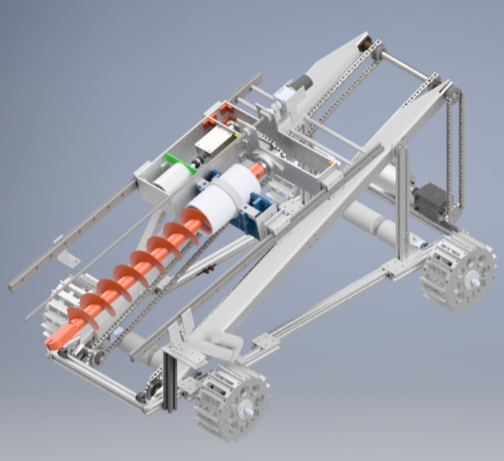
\includegraphics[width=0.5\linewidth]{09_Figures/final-cad.jpg}
	 \caption{Final Robot CAD Assembly}
	 \label{fig:final-cad}
	\end{figure}
	\FloatBarrier
	
	\subsubsection{Frame Section}
	
	The frame was designed to be lightweight and simple to modify (Figure \ref{fig:frame-cad}). It was constructed from 30mm by 30mm aluminum extrusions connected by corner brackets and flat mounting plates. Two vertical supports near the back connect the conveyor. The motor and gearbox that drive the conveyor were placed on the back extrusion. Only minor length changes were made to the frame between the preliminary design review and the final design. The final weight was under 4 kg.
	
	The wheel diameter was reduced to 7.875 inches since the rover was above the RMC height limit with the previous 30 cm diameter. The units were switched from metric to U.S. customary to aid in machining. The motor mount height was also decreased to lower the robot height.

	The final wheel design (Figure \ref{fig:wheel-cad}) was modified to be easier to fabricate. The first design had a lot of components that would make assembly challenging and could lead to points of failure. The wheel rim was eliminated to decrease weight. It did not provide much structural support, as most of the load is distributed through the sides of the wheel. The grousers are press fit and bolted into the wheel sides instead of using 3D printed spacers. The number of grousers was increased from twelve to eighteen. This increases traction and smoothes the ride. 

	VEX CIM motors were chosen to drive the wheels. The motors provide a maximum of 337 Watts. VEX parts are easy to assemble, as all the parts interface well together. Hex shafts were used over rotary shafts to increase the torque transmission between the axles and the wheels.
	
	
	\begin{figure}
	\centering
	\begin{minipage}{.49\textwidth}
	  \centering
	  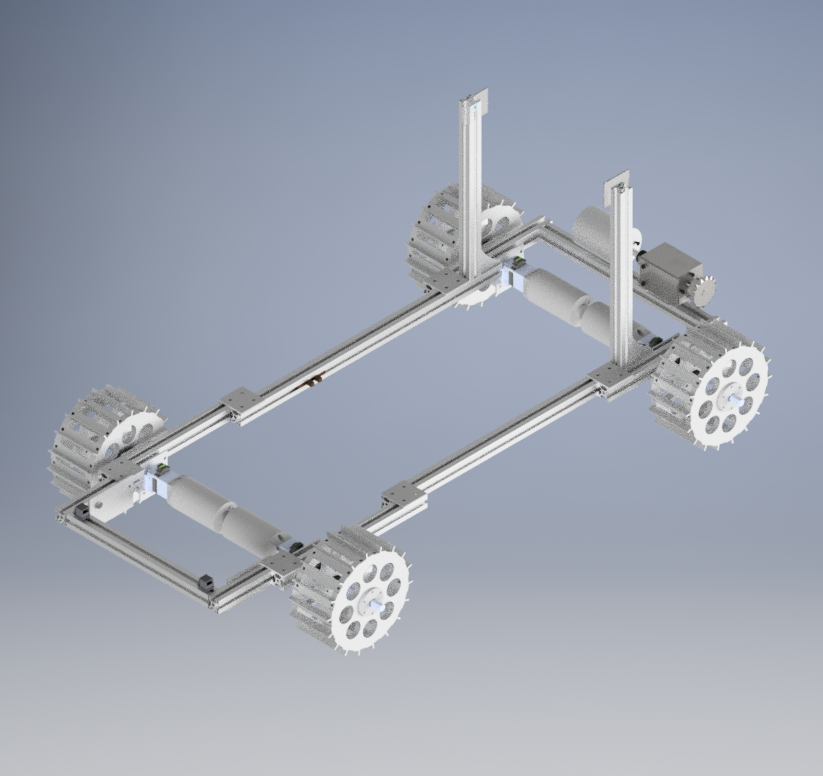
\includegraphics[width=.9\linewidth]{09_Figures/frame-cad.jpg}
	  \captionof{figure}{Final CAD Frame Assembly}
	  \label{fig:frame-cad}
	\end{minipage}
	\begin{minipage}{.49\textwidth}
	  \centering
	  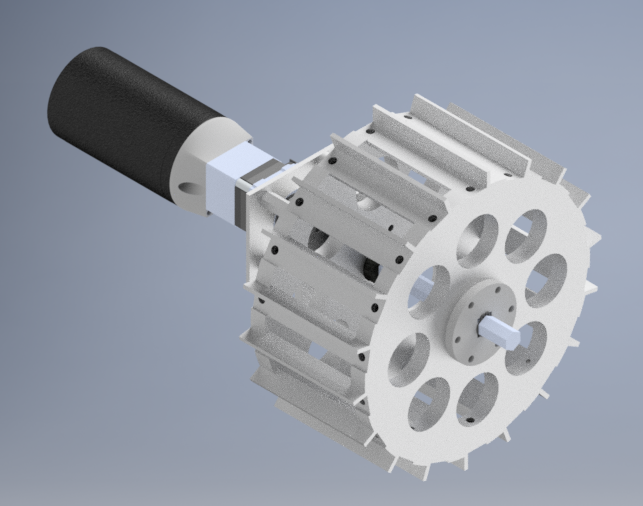
\includegraphics[width=.9\linewidth]{09_Figures/wheel-cad.jpg}
	  \captionof{figure}{Final Wheel Assembly}
	  \label{fig:wheel-cad}
	\end{minipage}
	\end{figure}
	
	
	\subsubsection{Excavation System}
	
	The auger must travel from its initial position to ground level during operation. The carriage, shown in Figure \ref{fig:carriage-cad}, supports the excavation system and contains the motor and gearbox that drive the auger. 
	
	\FloatBarrier
	\begin{figure}[h]
	\centering
	 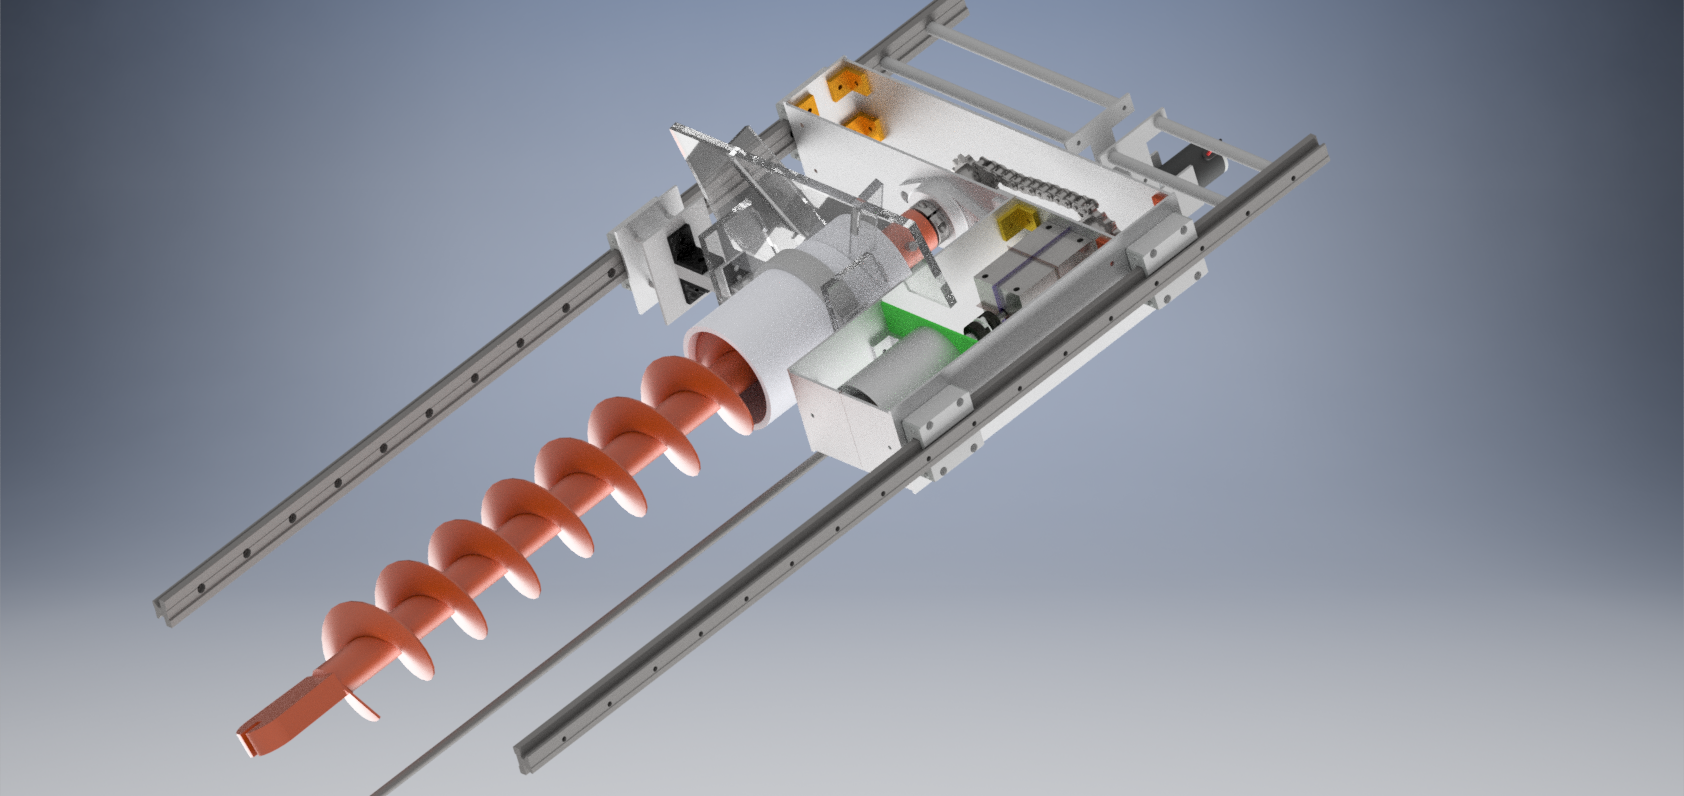
\includegraphics[width=0.8\linewidth]{09_Figures/carriage-cad.jpg}
	 \caption{Final Carriage CAD Assembly}
	 \label{fig:carriage-cad}
	\end{figure}
	\FloatBarrier
	
	A 2.2 horsepower motor and \#40 ANSI roller chain are used to drive the auger.  A flanged bushing and ball bearing support the auger from radial and thrust loads. Polycarbonate sheets cover the top and bottom of the carriage to protect the auger drive system from dust.
	
	The primary factors when selecting the auger were mass, digging length, power consumption, and ease of assembly. A 34 in. auger with a 4 in. radius was determined to travel deep enough to mine the icy gravel. 
	
	A PVC pipe was fitted to the auger to aid in regolith and gravel acquisition. The upward helical spiral on the auger funnels the gravel into the PVC pipe and can then be deposited into the collection bin. The tube is 8 in. long and has a 4.75 in. inner diameter and 5 in. outer diameter. 
	
	Due to size constraints, the auger must start the match constricted near the conveyor. Once the match begins, two linear actuators push the auger to its final angle of $75^\circ$ from the horizontal. A final angle of $60^{\circ}$ was desired, but it was not possible to fit an auger with the correct digging length at $60^\circ$ and fit within the RMC size constraints. The linear actuators and guide rails support the carriage as the auger travels to ground level. A lead screw driven by a motor provides the linear motion. The carriage and guide rails are attached directly to the frame.
	
	The fan (Figure \ref{fig:fan-cad}) is a system made of laser cut polycarbonate sheets that spreads out the icy regolith as it falls into the depositing system. This allows the material to be deposited evenly on the conveyor. Without the fan, the material would pile up in the center of the conveyor. 
	
	
	\subsubsection{Depositing}
	
	The gravel depositing system consists of a conveyor belt with standard \#40 ANSI roller chains and sprockets (Figure \ref{fig:con-cad}). It was determined that three supports were needed along the 4 feet conveyor belt to prevent roller chain deflection. A hollow rod was used for the middle support to reduce weight. Tensioners were attached at the bottom of each roller chain to allow for variable tension in case the roller chain deflected under heavy gravel loads. Flanged bushings were chosen to support the radial load on the rods since they were easy to assemble. The conveyor is driven from the back rod by a roller chain that runs to the frame and is connected to a motor and gearbox. The drive shaft is keyed to couple the two roller chains together and prevent misalignment. 
	
	\begin{wrapfigure}{l}{0.35\textwidth}
	\centering
	 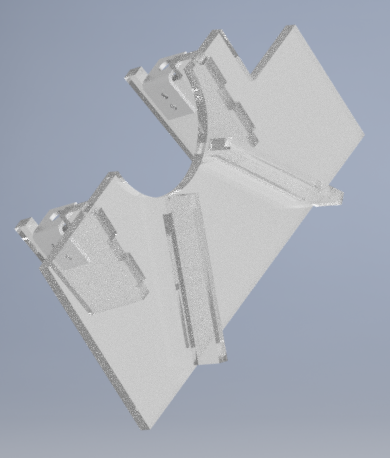
\includegraphics[width=0.3\textwidth]{09_Figures/fan-cad.jpg}
	 \caption{The Final Fan Assembly}
	 \label{fig:fan-cad}
	\end{wrapfigure}
	
	A nylon mesh was chosen as the conveyor belt so that BP-1 could be filtered out and no excess weight would be carried. The mesh is not shown in the CAD because it would be too computationally intensive to render.
	
	
	\subsubsection{Autonomy}
	
	The autonomy algorithm consists of a localization/mapping layer and a path planning layer. The localization and mapping layer interprets sensor data in order to determine the current location of the robot and maps the location of obstacles in the environment. An Extended Kalman Filter (EKF) Simultaneous Localization and Mapping (SLAM) algorithm was selected. Probabilistic SLAM algorithms are resilient to noisy sensor data and work well with low accuracy actuators. EKF SLAM was selected because of its ease of implementation and low computational cost compared to other methods, such as particle filter SLAM. The EKF SLAM algorithm incorporates data from the Kinect, camera, IMU, and encoders to update the location prediction.
	
	\begin{wrapfigure}{l}{0.35\textwidth}
	\centering
	 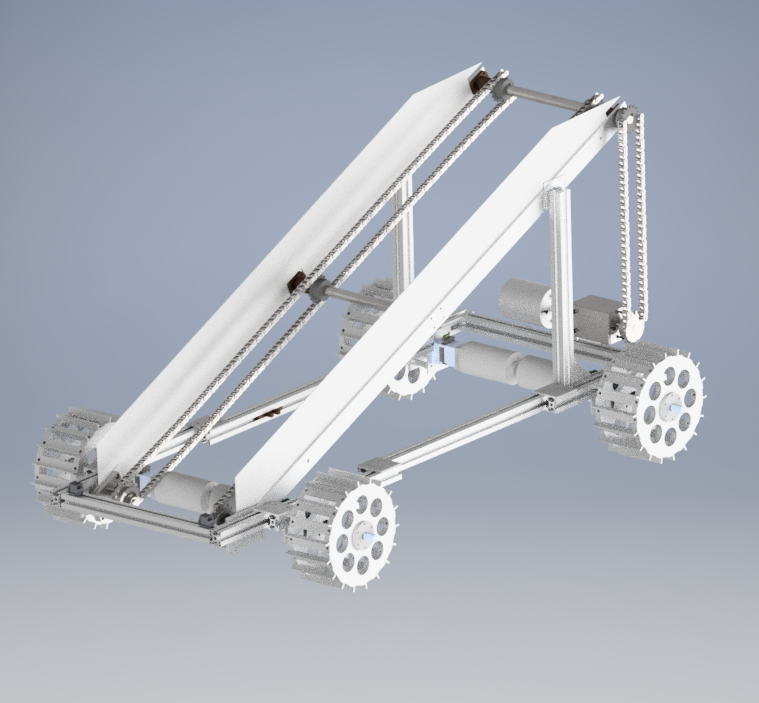
\includegraphics[width=0.9\linewidth]{09_Figures/conveyor-frame-cad.jpg}
	 \caption{Frame with Conveyor Belt Assembly}
	 \label{fig:con-cad}
	\end{wrapfigure}
	
	For camera-based localization, a webcam was utilized in conjunction with the AruCo package in OpenCV. A marker board comprised of markers from dictionary 0 of the AruCo package was created to mount on the collector bin. The algorithm converts each image into an adaptive threshold black-and-white version. From this version, it can detect the locations of the corners and compute the translation and rotational vectors of the markers relative to the robot reference frame. At the beginning of the competition run, the algorithm performs a scan of adaptive threshold values until a marker is detected to reduce noise from the dusty environment. If the marker is lost, the algorithm restarts the scan until it is detected again. 

	The Kinect is used to determine the location of rocks and ditches on the competition field. After removing the arena walls from the data, a random sample consensus (RANSAC) algorithm is applied to the ingested point-cloud to find the plane of the playing field. This plane is then subtracted from the point-cloud, leaving the large deviations in the sample. The location of these deviations is passed to the SLAM algorithm.

	Telemetry data is collected through a combination of the IMU and encoders. In order to improve accuracy of the encoder data, the acceleration from each drive wheel encoder is compared to the acceleration from the IMU to eliminate erroneous data from slippage.
	
	Based on the location of the robot and the environment map, the path planning algorithm determines the next control input for the robot to reach the desired location provided by the robot controller. The vector-field histogram algorithm was selected, which determines the next travel direction and velocity by building a polar histogram of obstacle density surrounding the robot.

	
	\subsubsection{Power Distribution}
	
	The requirements for power distribution were defined as follows:
	\begin{itemize}
	 \item All electronic devices on the robot must be powered at their nominal voltage (but not necessarily be on at all times during the competition)
	 \item Only one battery configuration can be used
	 \item Each electrical component on the robot must have at least a 20\% safety factor in each current-capacity aspect
	 \item The entire electrical system must be regulated by a red emergency shutoff switch
	 \item The batteries must satisfy the aggregate capacity requirements of all electrical subsystems (with a 20\% safety factor)
	\end{itemize}
	
	\FloatBarrier
	\begin{wrapfigure}{r}{0.4\textwidth}
	\centering
	 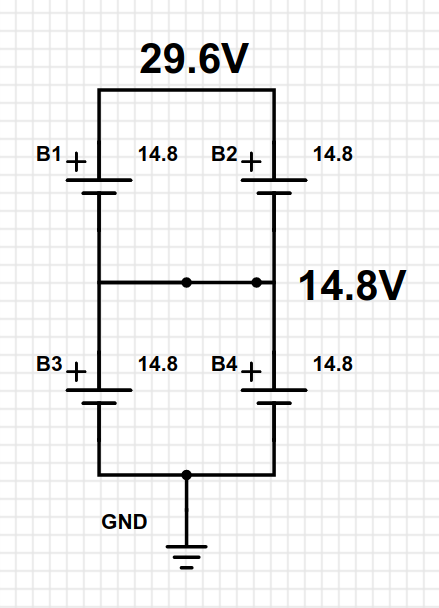
\includegraphics[width=0.8\linewidth]{09_Figures/power-config.jpg}
	 \caption{The schematic for the battery configuration of the robot. Note the two nodes at two different voltages.}
	 \label{fig:power-config}
	\end{wrapfigure}
	\FloatBarrier
	
	The robot is powered by four 4-cell (14.8V, nominal) Multistar LiPo batteries. LiPo batteries were used because of their high capacity-to-weight ratio. Two 16-Ah batteries are wired in parallel and two pairs of batteries are wired in series (See Figure \ref{fig:power-config}). The two front drive motors are powered by the bottom pair of batteries, and the two rear drive motors are powered by the other pair. The auger motor and the conveyor motor are each driven by all four batteries. This battery configuration enables efficient use of batteries for motors that are of differing voltage requirements; no costly, wasteful voltage transformers were required. 

	The front drive motor circuit, the rear drive motor circuit, and the conveyor and auger motor circuit each have an inline thermal circuit breaker; the drive circuit breakers are rated for 120A max, and the conveyor and auger circuit breaker for 150A max. This wiring configuration can help locate a wiring fault in the event of a short on any particular branch, and it utilizes small breakers instead of large, expensive breakers. 

	A red emergency stop button operates two main relays. One controls current flow through the rear drive motors, the conveyor, the auger, and the auxiliary electronics. The other controls the current flow through only the front drive motors. The relays are powered from one battery pair. The relay powering the front drive motors is a solid-state relay and is only rated for 100A, but the relay powering everything else is a gas-powered relay and is rated for upwards of 300A. 

	Boost converters are powered through both pairs of batteries. Each converter has a 90\% efficiency rating. They power 5- and 12-V devices on the robot, including all SoCs and sensors.
	
	Figure \ref{fig:power-dist} shows the detailed power distribution schematic. Each of the systems’ power usage, current usage, and expected duration of use are included in Table \ref{table:energy_budget}. The required amount of battery capacity was determined from this calculation table. 
	
	\FloatBarrier
	\begin{figure}[h]
	\centering
	 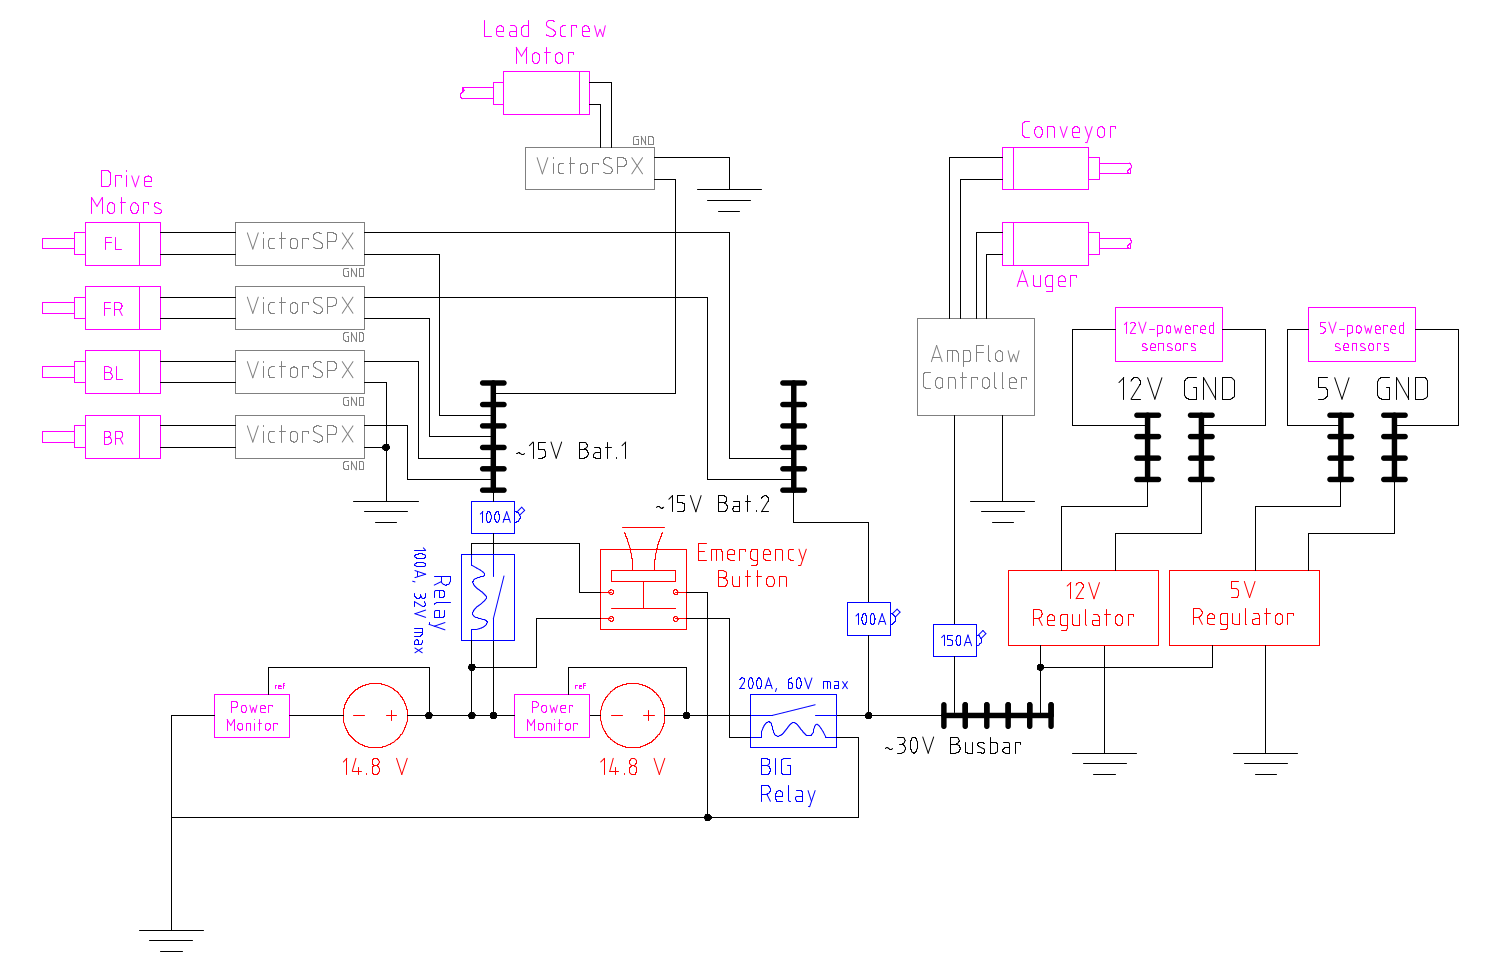
\includegraphics[width=1\linewidth]{09_Figures/power-distribution.jpg}
	 \caption{The broad-view scope of the robot’s power distribution scheme. This figure is adapted from a general wiring guide for team members, so it includes some niche specifications, such as the emergency button wiring scheme and the busbar and breaker configurations.}
	 \label{fig:power-dist}
	\end{figure}
	\FloatBarrier
	
	
	\subsubsection{Robot Controller}
	
	The final robot controller splits hardware and software capabilities across multiple devices. Most sensors and all output signals come from the real-time power of the BeagleBone Blue. The only application running on the BeagleBone Blue abstracts its connections to the real world by interpreting its raw sensor inputs and publishing their information in useful message formats. It then accepts a message for motor output control to abstract the connection to the motors.The implementation of this software in ROSMOD allows for the application to easily be configured and deployed to any BeagleBone and seamlessly integrate into any previous code.
	
	The UP Board acts as the main processing hub. It interfaces with the Kinect and camera via USB to provide fast access to their raw data. The processing of the depth data, camera images, and path planning all takes place on the UP Board. Each ability is implemented in a separate component with a set interface for communication with other components. At the top level, a state machine dictates what the robot should be doing at any moment. It takes in all of the processed sensor information to make decisions about when an operation should be performed and publishes this state to the other components.
	
	The implementation of each ability of the robot as a separate component in ROSMOD allows for different abilities to be quickly enabled, disabled, and tested. Each component has a set interface and does not care which other component is using its interface. This allows for easy simulation of code processing. Sensor inputs can be simulated and allow for the observation of the response of the real software.

	
	\subsubsubsection{Operator Controller}
	
	The primary responsibility of the operator station is to provide the operators with real time information about the robot and accept operator commands. The operator controller is based entirely in the ROS visualizer (rviz). The use of standard ROS messages throughout the robot controller allows rviz to quickly provide a visualization of critical robot sensors and controls. The autonomy controller takes commands from the operator interface as to whether it should be operating autonomously, teleoperated, or disabled. The robot controller then disables the command messages from autonomy controller and enables the teloperated control nodes. The teleoperated node on the command station takes in joystick data and on-screen commands and converts them to robot subsystem commands. This allows the operator control to seamlessly take over control from the autonomy system without additional overhead.
	
	
	
	\subsection{Critical Design Review}
	
	On March 5, 2018, the Vanderbilt Robotics executive board met with the team’s faculty adviser for a final design review. The CAD assembly of each subsystem was analyzed for its functionality and potential failure points. The team was cleared to move on to the fabrication and assembly phase and to begin purchasing parts. 
	
	
	


	
\end{document}
